% Anonymized submission to the OFF-Grid workshop (MICCAI 2026 satellite).
% Uses the same LNCS class file shipped with the official MICCAI template.

\documentclass[runningheads]{llncs}

%
\usepackage[T1]{fontenc}
% T1 fonts will be used to generate the final print and online PDFs,
% so please use T1 fonts in your manuscript whenever possible.
% Other font encodings may result in incorrect characters.
%
\usepackage{graphicx,verbatim}
% Used for displaying a sample figure. If possible, figure files should
% be included in EPS format.
%
% If you use the hyperref package, please uncomment the following two lines
% to display URLs in blue roman font according to Springer's eBook style:
%\usepackage{color}
%\renewcommand\UrlFont{\color{blue}\rmfamily}
%\urlstyle{rm}

\usepackage{booktabs}
\usepackage{amsmath,amssymb}
\usepackage{multirow}
\usepackage{microtype}
\usepackage{xcolor}

\graphicspath{{figures/}}

\begin{document}


\title{CONFETTI: CONvolutional FibEr TracT Inference
with Multi-Resolution Graphs}
\titlerunning{CONFETTI: Convolutional Fiber Tract Inference}

\author{Anonymized Authors}
\authorrunning{Anonymized Author et al.}
\institute{Anonymized Affiliations \\
    \email{email@anonymized.com}}

\maketitle

\begin{abstract}
Per-tract-bundle mean summaries are commonly used for diffusion MRI based
white-matter (WM) microstructure analyses to reduce the dimensionality of
the data, but collapsing each tract to a set of scalars (one per diffusion
metric) discards the within-tract spatial structure and vastly reduces
spatial localization of effects. We introduce \textbf{CONFETTI}
(\textbf{CON}volutional \textbf{F}ib\textbf{E}r \textbf{T}rac\textbf{T}
\textbf{I}nference), a WM analysis pipeline built around three
components: (i) a hierarchical multi-resolution neighborhood graph over
parametrized fiber axes that retains within-tract spatial structure and
between-tract proximity; (ii) an implicit-neural-representation-based
imputation for missing diffusion tract profiles; and (iii) a Graph
Convolutional Network (GCN) analysis including per-tract/node/covariate
interpretable attribution. We evaluate CONFETTI with three structurally
distinct architectures: 1) single-level GCN, 2) multi-scale parallel-branch
concatenation, 3) hierarchical Graph U-Net, in a study of WM microstructure
in infants with Down syndrome (DS). We investigate DS classification as
well as prediction of later outcome scores. We compare
CONFETTI against per-tract mean baselines (logistic regression and
XGBoost). Our results show that while the classification performance is
comparable between baselines and the three GCN models, the attribution
results show a spatially finer pattern, as well as the emergence of the
anterior commissure (AC) as a tract of higher relevance in DS. It is the
top-ranked tract for the GCN-based models, while neither baseline lists it
in its highly ranked tracts. Via several follow-up experiments, we show
that this spatial finding is robust, and that it requires CONFETTI's
within-tract spatial coupling to emerge, providing a showcase result for
the proposed convolutional tract analysis with CONFETTI over traditional
per-tract mean summaries.

\keywords{Graph Convolutional Network \and Diffusion MRI
  \and Fiber Tractography \and Spatial Attribution \and Down Syndrome.}
\end{abstract}


\section{Introduction}

White matter (WM) fiber based microstructure analysis from diffusion MRI data typically reduces 
fiber bundles to one number per diffusion metric: a tract-average
Fractional Anisotropy (FA), or Neurite Density Index (NDI) or similar~\cite{ref_zhang}.
This compression is convenient for traditional statistical analyses and
classifiers~\cite{ref_chen,ref_breiman} but
deliberately removes the along-tract spatial profile reducing the spatial localization of effects~\cite{ref_yeatman,ref_cohort}.
Fiber-bundle methods such as the atlas based
UNC-Utah NA-MIC DTI framework~\cite{ref_verde2014}
or similar ones such as the Automated Fiber Quantification
family~\cite{ref_yeatman} generate along-tract, per-node diffusion metric profiles. Current profile analysis methods focus on per-tract analyses, and no all-tract/whole-brain methods exist that operate on these 1D profiles
\emph{jointly across tracts}, treating the whole white-matter representation
as a single geometric object.

\paragraph{CONFETTI:}
We address this gap with \textbf{CONFETTI} (Convolutional Fiber Tract
Inference), a multi-resolution graph convolutional pipeline for
WM microstructure analysis combining (1) a hierarchical
neighborhood graph over parametrized fiber axes with nested levels
$L_0,\dots,L_5$ shared across subjects, that captures both within-tract
continuity and between-tract proximity, (2) a per-subject
implicit neural representation (INR)-based imputation~\cite{ref_sitzmann} for missing
profiles, and (3) a GCN analysis stack with an out-of-fold
interpretable attribution back-end (permutation
importance~\cite{ref_breiman}, integrated gradients~\cite{ref_sundararajan}, and
sparse GNNExplainer mask~\cite{ref_ying}). CONFETTI is
architecture-agnostic; we compare here three structurally distinct
GCN heads: a single-level GCN~\cite{ref_kipf}, a multi-scale parallel-branch
concatenation~\cite{ref_hamilton,ref_velickovic}, and a hierarchical Graph
U-Net~\cite{ref_gao}.

\paragraph{Application:}
We evaluate CONFETTI in a study of WM microstructure in
infants with Down syndrome (DS), a cohort that offers a methodological
stress test: per-tract mean baselines already saturate the classification
AUC, so any added value from CONFETTI must come from
\emph{interpretation}. We benchmark CONFETTI against logistic regression
and XGBoost on per-tract DTI/NODDI means under matched nested
cross-validation on (a) DS classification and (b) prospective regression
of 24-month behavioral outcomes from 6-month
imaging, then run focused validation experiments on the divergent finding.


\paragraph{Contributions:}
(i)~\textbf{CONFETTI}, a multi-resolution graph convolutional pipeline for
WM microstructure analysis with INR-based per-subject imputation and an
out-of-fold GCN-based attribution stack.
(ii)~Three GCN instantiations (single-level, multi-scale concat, Graph
U-Net) that share the same CONFETTI front-end and attribution back-end,
making cross-architecture comparison meaningful.
(iii)~A DS showcase in which CONFETTI matches strong per-tract mean
baselines in accuracy while the \emph{anterior commissure} (AC) emerges
as a top-ranked spatial finding that neither baseline lists in its highly
ranked tracts; follow-up experiments establish the finding as biological
signal rather than methodological artifact.
(iv)~A prospective-regression head showing that the same dominant spatial
pattern predicts 24-month behavioral outcomes from 6-month imaging.

\begin{figure}[bth]
  \centering
  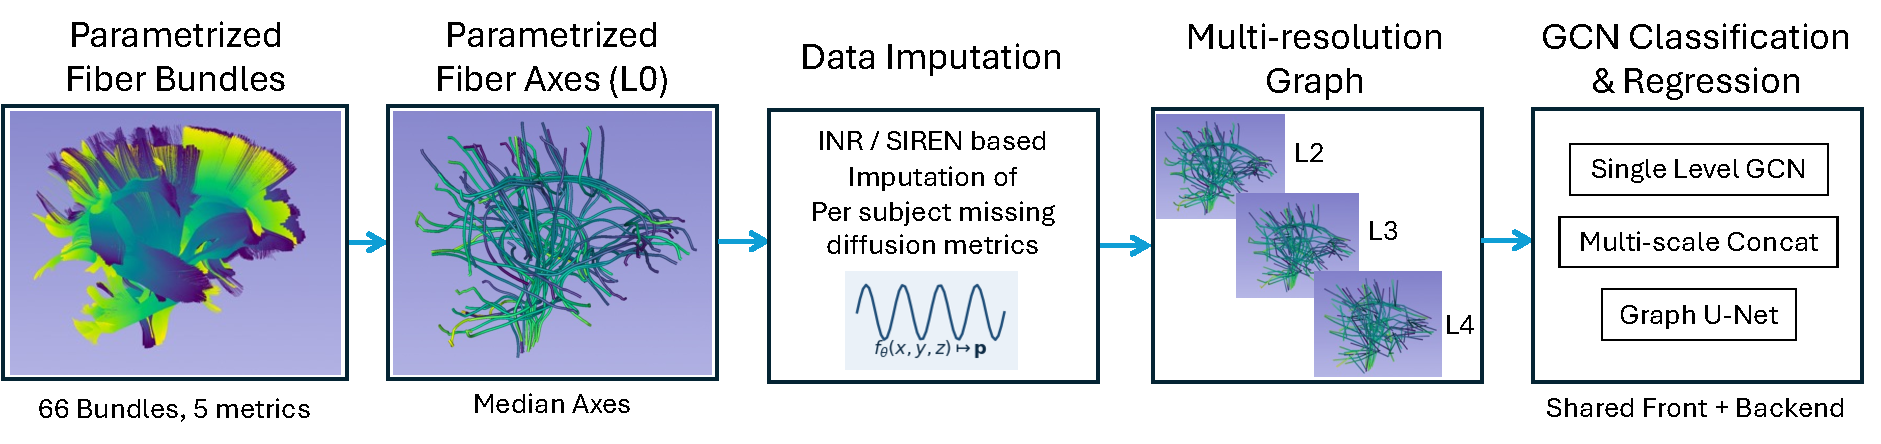
\includegraphics[width=\linewidth]{Fig_Pipeline2.pdf}
  \caption{CONFETTI overview. (a) Per-subject parametrized fiber bundles
  ($66$ tracts, $5$ DTI/NODDI metrics); (b) per-tract parametrized fiber
  axes at $L_0$, computed as a median location each bundle's fibers;
  (c) SIREN per-subject INR imputation of missing profiles;
  (d) hierarchical multi-resolution neighborhood graph ($L_2$, $L_4$, $L_5$
  shown); (e) three GCN heads sharing
  the CONFETTI front-end and attribution back-end.}
  \label{fig:pipeline}
\end{figure}

\section{The CONFETTI Pipeline}

\subsection{From fiber tracts to multi-resolution graphs}
Figure~\ref{fig:pipeline} summarizes the pipeline; the remainder of this
section details each component in turn.

For each of $66$ pre-segmented white-matter tracts, we compute a 1D parametrized fiber axis 
by binning per-subject fiber
points along their canonical arclength and taking the per-bin median, with
end-clipping for outliers. A neighborhood graph is built over the
concatenation of all axis points: two points are connected if they are
adjacent on the same axis or within $1.5\times$ the median nearest
cross-tract distance, with edge weights $\exp(-d^2/\sigma^2)$. From the
finest graph $L_0$ ($\sim$4{,}766 nodes) we recursively subsample to
produce $L_1,\dots,L_5$ while preserving each tract's endpoints. This
hierarchy is computed once and shared across subjects.

\subsection{Per-subject node features and INR imputation}

Fiber QC procedures commonly remove 5-10\% of fiber profiles resulting in uneven 
profile coverage which needs correction via data imputation. 
At each axis node we attach five diffusion metrics (FA, RD, AD, NDI, ODI)
and four spatial features ($x,y,z,\ell$) for a $9$-D input. 
Any missing profile data were imputed using an implicit neural representation (INR) model using
SIREN~\cite{ref_sitzmann} activation functions ($200$ epochs, $\omega_0\!=\!10$). Per-fold
training-set statistics are used so that the imputation
respects the nested-CV split. Three subject-level covariates (sex,
gestational age at birth, DWI artifact level) are mean-imputed per
fold and concatenated to the graph embedding before the MLP head, keeping
demographics separable from the spatial pattern under attribution. We compare the INR imputation versus traditional baselines (kNN with 5 and 10 neighbors, linear, mean, median imputation).

\subsection{GCN architectures for CONFETTI}

CONFETTI is architecture-agnostic at the head; we instantiate it with three
GCN architectures whose inductive biases differ significantly.
\textbf{Single-level GCN} is a two-layer Kipf-Welling GCN at a single, relatively coarse
 level only (here L3).
\textbf{Multi-scale concat} runs an independent two-layer GCN at two levels (here L2 and L3)
in parallel and concatenates global-pooled embeddings before the head.
\textbf{Hierarchical Graph U-Net} replaces dynamic pooling with the fixed
index hierarchy above (from L2 to L3 to L4): a GCN block per encoder level, scatter-unpool with
skip connections in the decoder, and global mean+max pool of the finest
decoder level into the output head. Best models are selected on inner-fold
validation AUC (or negative-MAE for regression).

\subsection{Attribution stack}

For each architecture we compute three complementary attributions:
out-of-fold permutation importance~\cite{ref_breiman} for tracts, per-node
positions, covariates, and (in regression) per-target; integrated gradients
on the input feature tensor~\cite{ref_sundararajan}; and a sparse
GNNExplainer mask~\cite{ref_ying} per held-out subject. The permutation
importance metric is the drop in held-out AUC (or rise in held-out MAE for
regression) when a feature group is shuffled across subjects in the
outer-CV test fold. Crucially this is computed inside the nested-CV loop,
so the model used for attribution has never seen the test subjects.

\section{Application: Infant Down Syndrome Study}

\subsection{Dataset and cross-validation protocol}

We evaluate on an infant Down syndrome (DS) cohort~\cite{ref_cohort} with imaging at
6 months and outcome assessment at 24 months
with 59 infants with DS and 68 control infants. Five diffusion metrics are assessed: FA, RD (Radial Diffusivity), AD (Axial Diffusivity), NDI, and ODI (Orientation Dispersion Index). For the
prospective regression we predict scores from a behavioral assessment measured at 24 months of age, specifically the Vineland-III Daily Living Skills.

All experiments use a stratified 5-fold cross-validation
repeated 3 times with inner-fold model selection.


\begin{table}[bt]
\centering
\caption{Down syndrome classification: held-out CV AUC and F1 with
covariates concatenated at the head. Baselines compute per-tract DTI/NODDI
means; CONFETTI uses per-node features under the multi-resolution graph
pipeline. Numbers are mean $\pm$ std over $15$ outer folds ($5\times 3$
repeats), best dropout per model.}
\label{tab:cls}
\begin{tabular}{lcc}
\toprule
Method & AUC & F1 \\
\midrule
LogReg (per-tract means) & $1.000\pm 0.000$ & $0.994\pm 0.015$ \\
XGBoost (per-tract means) & $0.983\pm 0.018$ & $0.921\pm 0.052$ \\
\midrule
CONFETTI - Single-level GCN (L3) & $0.913\pm 0.125$ & $0.809\pm 0.250$ \\
CONFETTI - Multi-scale concat (L2+L3) & $0.931\pm 0.084$ & $0.820\pm 0.128$ \\
CONFETTI - Graph U-Net (L2-L4) & $\mathbf{0.940\pm 0.106}$ & $\mathbf{0.888\pm 0.093}$ \\
\bottomrule
\end{tabular}
\end{table}

\subsection{Imputation evaluation}

We evaluated the INR imputation on a held-out subset of $34$ subjects with
complete data by removing $7$ random tracts per subject and
reconstructing them from the rest. Normalized mean absolute error (NMAE) was lowest for
INR/SIREN ($0.520$), followed by kNN-$10$ ($0.576$, $+11\%$ vs INR),
kNN-$5$ ($+16\%$), linear ($+30\%$), median ($+34\%$), and mean ($+37\%$). The INR/SIREN imputation outperforms all baselines significantly (p<0.001).

\subsection{Classification: CONFETTI is close to baselines, but with
different attribution}

Table~\ref{tab:cls} summarizes the held-out classification performance.
Logistic regression on per-tract means saturates at a near perfect performance
$\mathrm{AUC} = 1.000, \mathrm{F1} = 0.994$; XGBoost reaches $0.983 / 0.921$. All
three CONFETTI models land a bit lower, between $0.913$ and $0.940$, with the
Graph U-Net at the upper end. The gap is
relatively small, likely due to the larger complexity of the GCN models. 



\begin{figure}[tb]
  \centering
  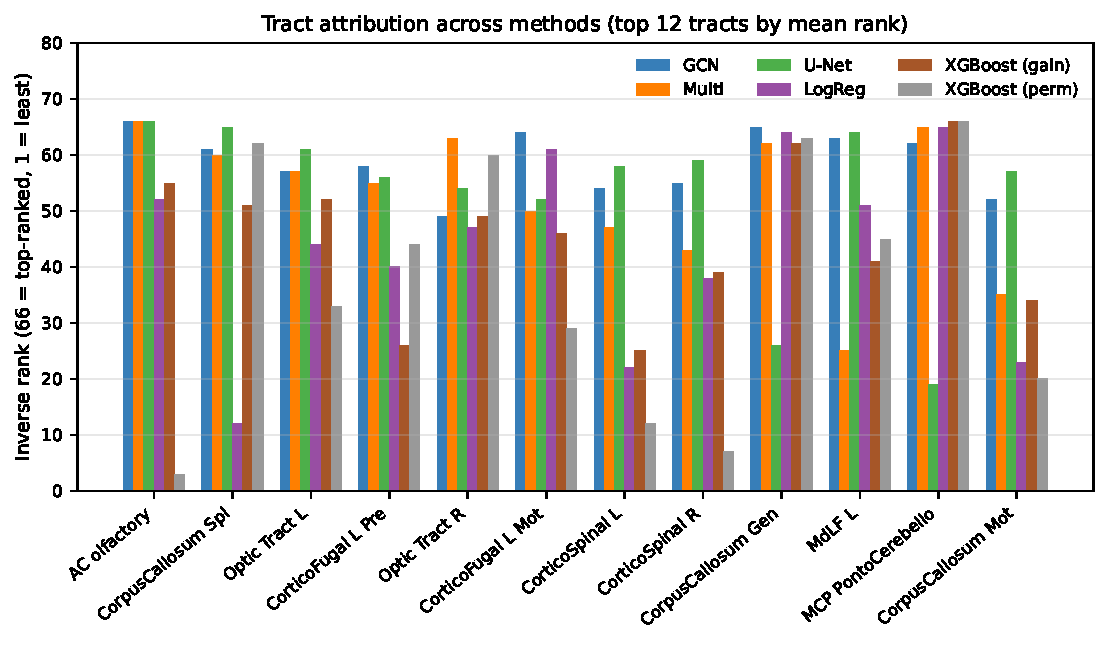
\includegraphics[width=\linewidth]{fig_attr_ranking.pdf}
  \caption{Cross-method tract attribution. Per-method inverse rank (66 minus
  rank) for the top tracts. The three CONFETTI models agree on
  the AC olfactory at rank 1; the baselines rank the MCP 
   and CC Lateral Genu tracts highest. The MCP and CC Lateral Genu tracts appear in $\geq 5/6$ top-10 lists.}
  \label{fig:rank}
\end{figure}

Per-tract attribution tells a different story for the baselines and the GCN models. Figure~\ref{fig:rank} compares
the inverse rank (highest bar = top-ranked tract) of the top ranking tracts. The two baselines put the \emph{Mid Cerebellar Pontine (MCP) tract} at rank 1,
with the \emph{Corpus Callosum (CC) Lateral Genu tract} a close second. In contrast, all three CONFETTI
permutation rankings put the \emph{Anterior Commissure (AC) olfactory} at rank 1 by a wide margin,
while still flagging the MCP tract as a secondary
contributor. Furthermore, spearman rank correlation across all $66$ tracts is $0.64$
between the two baselines,  but only (at most) $0.34$ between any CONFETTI
instantiation and any baseline.


\subsection{Validating CONFETTI's divergent finding}

We ran five experiments to establish whether CONFETTI's AC olfactory tract
importance is a biological signal or a methodological artifact.

\begin{figure}[bt]
  \centering
  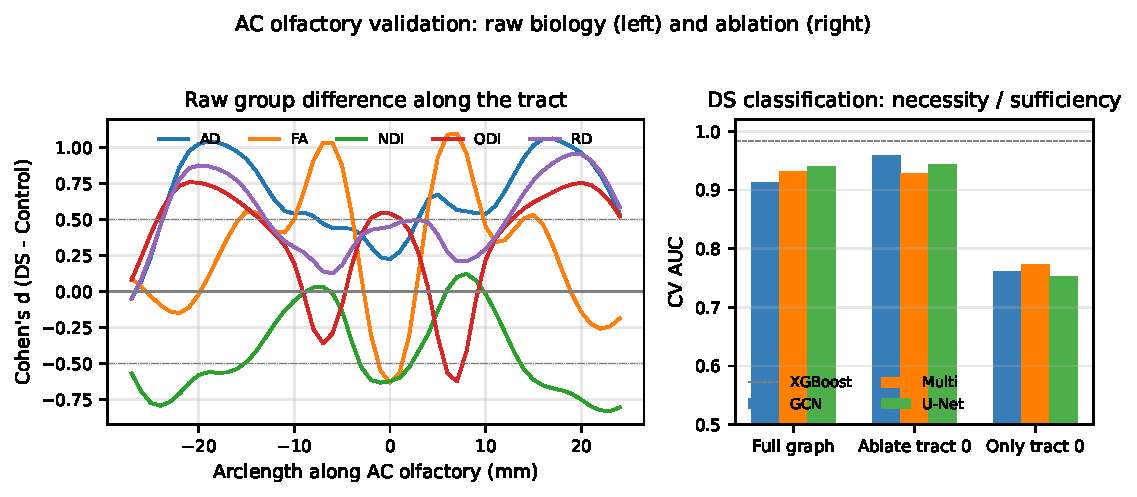
\includegraphics[width=\linewidth]{fig_acolf_validation.pdf}
  \caption{Validation of the AC olfactory finding. Left: per-node Cohen's
  $d$ along AC olfactory for each diffusion property; horizontal dotted
  lines mark $|d|=0.5$. Right: classification AUC with the full graph,
  AC olfactory ablated, and only AC olfactory retained; dashed line is
  XGBoost.}
  \label{fig:valid}
\end{figure} 

\paragraph{(1,2) Raw biology and per-property channels.}
Two-sample $t$-tests at each of the $52$ AC olfactory nodes per
property ($260$ tests, FDR-corrected~\cite{ref_benjamini})
yield $174/260$ significant at $q<0.05$, and all $52$ nodes are
significant for at least one property; peak per-node Cohen's $d$ reaches
$+1.10$ for AD and $+1.09$ for FA (Fig.~\ref{fig:valid}, left). While the overall 
direction (AD$\uparrow$, RD$\uparrow$, NDI$\downarrow$, ODI$\uparrow$)
matches the hypomyelination + reduced-neurite-density signature reported
in DS cohorts~\cite{ref_cohort,ref_saini2025white,ref_carducci}, the group differences invert direction for FA, ODI, and NDI along the tract. 
This effect inversion cannot be captured by tract means and is likely one of the reasons the baselines do not rank the AC olfactory at the top.   

Restricting the OOF permutation
to AC olfactory and shuffling one property at a time isolates AD ($+0.048$
gcn, $+0.036$ unet) and RD as the predictive drivers; NDI and ODI
contribute near zero. CONFETTI's attribution at the AC olfactory tract
therefore loads on the axial and radial diffusivity channels.

\paragraph{(3,4) Necessity and sufficiency.}
Replacing AC olfactory's per-node values with the training-fold mean does
not hurt classification (CV AUC $0.913\to 0.959$ gcn, $0.931\to 0.929$
multi, $0.940\to 0.944$ unet): the models redistribute information across
the remaining $65$ tracts, consistent with the expected brain-wide DS pathology. Training
on AC olfactory alone reaches $0.761/0.774/0.752$ (gcn/multi/unet),
well above chance from the $\leq 52$ axis points (Fig.~\ref{fig:valid},
right). AC olfactory is therefore informative but redundant for
classification.

\paragraph{(5) Within-tract spatial peak.}
Aggregating the OOF GNNExplainer per-DS-subject masks places the spatial peak
at arclength $+13$\,mm across all three CONFETTI architectures, with
$\geq 1.6\times$ activation versus other-tract nodes. This convergence
under a different attribution mechanism than (1-4) indicates a likely stable
spatial signal rather than a permutation artifact.


\subsection{Predictive regression: 6-month imaging predicts later outcomes}

We applied CONFETTI to a regression of the 24-month Vineland Daily Living Skills
standardized scores. The performance of the regression is quite strong.
Table~\ref{tab:reg} shows held-out Pearson $r$ for
the Graph U-Net instantiation (the strongest CONFETTI head on this task)
against the two baselines. CONFETTI outperforms both baselines.

\begin{table}[t]
\centering
\caption{6 month imaging predicting 24 month outcomes. Pearson $r$
on held-out folds (mean over 3x5 folds; std in parentheses). \textbf{Bold} =
best of row.}
\label{tab:reg}
\fontsize{8.5}{10}\selectfont
\begin{tabular}{lccc}
\toprule
V24 outcome & Ridge baseline & XGBoost baseline & Graph U-Net \\
\midrule
Vineland Daily Living Skills         & $0.32\,(.19)$ & $0.48\,(.12)$ & $\mathbf{0.51\,(.13)}$ \\
\bottomrule
\end{tabular}
\end{table}

\paragraph{Per-target attribution.}
Figure~\ref{fig:dailyliving} shows CONFETTI's OOF tract permutation
importance for the Graph U-Net head. AC olfactory is the top-attributed
tract for the prediction, with a $\sim\!4\times$ gap over the next-largest. The fold-wise std is wide (0.72), reflecting that the effect is very concentrated in some folds and modest in others — but the mean remains clearly the largest of any tract. The left optic tract is the strongest secondary contributor.

The same OOF protocol applied to the three covariates shows that sex has
a predictive signal for the Daily Living score ($+0.212$), roughly half
the AC olfactory tract effect. Contributions from gestational age at
birth are much smaller and from DWI artifacts essentially zero.

\begin{figure}[tb]
  \centering
  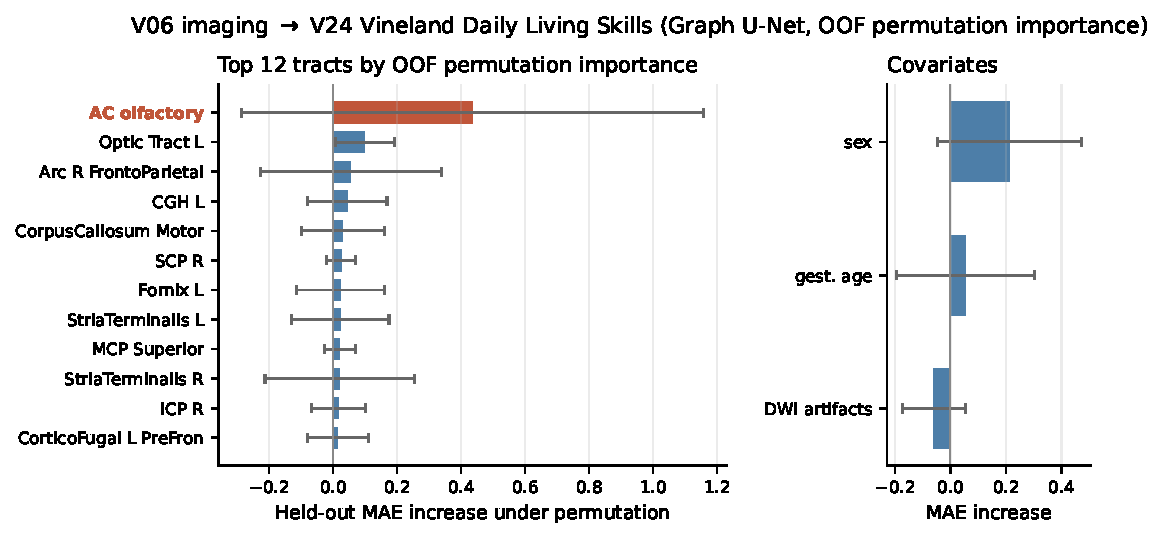
\includegraphics[width=0.99\linewidth]{fig_dailyliving_importance.pdf}
  \caption{CONFETTI per-target tract attribution for the 6-month diffusion $\rightarrow$ 24-month behavior
  predictive regression (Graph U-Net). }
  \label{fig:dailyliving}
\end{figure}


\section{Discussion}

Under matched out-of-fold cross-validation, CONFETTI's top-ranked tract
differs from that of the per-tract-mean baselines: CONFETTI puts the AC
olfactory tract at rank 1, while the tract mean methods put the middle cerebellar peduncle at rank 1 with the
AC olfactory outside of the top-10. The follow-up experiments establish
this as biological signal rather than artifact, and the same tract
dominates the predictive outcome regression. The likely reasons the baselines miss this finding: (1) group differences invert direction along the tract which cannot be captured by tract means, (2) the AC olfactory has also particularly sharp group differences that
mean-pooling averages away. Other architecture-independent consensus tracts remain visible
in CONFETTI's attribution. 

The AC olfactory tract is generally understudied. Almost no single diffusion MRI study quantifies the AC olfactory on its own. When the AC is studied, quantification is limited to the AC as one bundle or to the larger posterior part. The results here show that particularly for DS studies, the AC olfactory tract should be included. This diffusion tract finding is supported by prior literature where severe, broad-based olfactory impairment affecting threshold detection, odor discrimination, and odor identification are observed in DS~\cite{ref_brozzetti2023,ref_cecchini2016}.

It is worthwhile to note that the left and right optic tract are
consistent secondary contributors. These tracts show an opposite directional signature to the AC olfactory tract: higher FA and lower RD/ODI indicating a seemingly more coherent microstructure pattern in DS, which is a biologically surprising finding. On the other hand, in a neurodevelopmental context, this pattern of diffusion MRI differences could also be interpreted as atypical development due to sparser fiber populations or thinner axons.

\section{Conclusion}

We introduced CONFETTI, a white-matter analysis framework that treats the whole tractography as a single off-grid geometric object rather than a set of per-tract means. Its methodological contributions are (i) a hierarchical multi-resolution neighborhood graph over parametrized fiber axes preserving within-tract and between-tract structure in one shared hierarchy, (ii) a per-subject INR imputation for missing diffusion profiles that outperforms kNN, linear, mean and median baselines, and (iii) an architecture-agnostic GCN back-end with a nested-CV out-of-fold attribution stack. Together these components enable joint cross-tract attribution that recovers spatial signals per-tract-mean baselines do not reveal, illustrated here by the infant DS AC olfactory finding.
%\section{Acknowledgments}
%Blinded/Anonymous.

\begin{thebibliography}{18}

\bibitem{ref_kipf}
Kipf, T.N., Welling, M.: Semi-supervised classification with graph convolutional
networks. In: International Conference on Learning Representations (ICLR) (2017)

\bibitem{ref_hamilton}
Hamilton, W., Ying, R., Leskovec, J.: Inductive representation learning on large
graphs. In: Advances in Neural Information Processing Systems (NeurIPS),
pp.~1024-1034 (2017)

\bibitem{ref_verde2014}
Verde, A.R., Budin, F., Berger, J.-B., Gupta, A., Farzinfar, M., Kaiser, A.,
Ahn, M., Johnson, H., Matsui, J., Hazlett, H.C., Sharma, A., Goodlett, C.,
Shi, Y., Gouttard, S., Vachet, C., Piven, J., Zhu, H., Gerig, G., Styner, M.:
UNC-Utah NA-MIC framework for DTI fiber tract analysis. Frontiers in
Neuroinformatics \textbf{7}, 51 (2014)

\bibitem{ref_velickovic}
Veli\v{c}kovi\'c, P., Cucurull, G., Casanova, A., Romero, A., Li\`{o}, P.,
Bengio, Y.: Graph attention networks. In: International Conference on Learning
Representations (ICLR) (2018)

\bibitem{ref_gao}
Gao, H., Ji, S.: Graph U-Nets. In: International Conference on Machine
Learning (ICML), pp.~2083-2092 (2019)

\bibitem{ref_ying}
Ying, R., Bourgeois, D., You, J., Zitnik, M., Leskovec, J.: GNNExplainer:
generating explanations for graph neural networks. In: Advances in Neural
Information Processing Systems (NeurIPS), pp.~9244-9255 (2019)

\bibitem{ref_sundararajan}
Sundararajan, M., Taly, A., Yan, Q.: Axiomatic attribution for deep networks.
In: International Conference on Machine Learning (ICML), pp.~3319-3328 (2017)

\bibitem{ref_breiman}
Breiman, L.: Random forests. Machine Learning \textbf{45}(1), 5-32 (2001)

\bibitem{ref_chen}
Chen, T., Guestrin, C.: XGBoost: a scalable tree boosting system. In:
Proceedings of the 22nd ACM SIGKDD International Conference on Knowledge
Discovery and Data Mining, pp.~785-794 (2016)

\bibitem{ref_sitzmann}
Sitzmann, V., Martel, J.N.P., Bergman, A.W., Lindell, D.B., Wetzstein, G.:
Implicit neural representations with periodic activation functions. In:
Advances in Neural Information Processing Systems (NeurIPS) (2020)

\bibitem{ref_yeatman}
Yeatman, J.D., Dougherty, R.F., Myall, N.J., Wandell, B.A., Feldman, H.M.:
Tract profiles of white matter properties: automating fiber-tract quantification.
PLoS ONE \textbf{7}(11), e49790 (2012)

\bibitem{ref_zhang}
Zhang, H., Schneider, T., Wheeler-Kingshott, C.A., Alexander, D.C.: NODDI:
practical in vivo neurite orientation dispersion and density imaging of the
human brain. NeuroImage \textbf{61}(4), 1000-1016 (2012)

\bibitem{ref_basser}
Basser, P.J., Pierpaoli, C.: Microstructural and physiological features of
tissues elucidated by quantitative-diffusion-tensor MRI. Journal of Magnetic
Resonance B \textbf{111}(3), 209-219 (1996)

\bibitem{ref_cohort}
Anonymized for double-blind review: pediatric Down Syndrome neuroimaging
cohort study. [Reference details withheld for double-blind review; will be
inserted in the camera-ready version.]

\bibitem{ref_carducci}
Carducci, F., Onorati, P., Condoluci, C., Di Gennaro, G., Quarato, P.P.,
Pierallini, A., Sara, M., Miano, S., Cornia, R., Albertini, G.: Whole-brain
voxel-based morphometry study of children and adolescents with Down syndrome.
Functional Neurology \textbf{28}(1), 19-28 (2013)

\bibitem{ref_saini2025white}
Saini, F., Ivain, P., Idris, M., Wells, J., Bianchi, L., Tamayo-Elizalde, M.,
Dell'Acqua, F., Strydom, A.: White matter trajectories in Down syndrome
and Alzheimer's disease: insights from diffusion tensor-based morphometry.
Alzheimer's \& Dementia \textbf{21}(6), e70382 (2025)

\bibitem{ref_benjamini}
Benjamini, Y., Hochberg, Y.: Controlling the false discovery rate: a practical
and powerful approach to multiple testing. Journal of the Royal Statistical
Society B \textbf{57}(1), 289-300 (1995)

\bibitem{ref_cecchini2016}
Cecchini, M.P., Viviani, D., Sandri, M., et al.: Olfaction in people with
Down syndrome: a comprehensive assessment across four decades of age.
PLoS One \textbf{11}(1), e0146486 (2016)

\bibitem{ref_brozzetti2023}
Brozzetti, L., Scambi, I., Bertoldi, L., et al.: RNAseq analysis of
olfactory neuroepithelium cytological samples in individuals with Down
syndrome compared to euploid controls: a pilot study. Neurological
Sciences \textbf{44}(3), 919-930 (2023)

\end{thebibliography}

\end{document}
